\documentclass[cjk,slidestop,compress,mathserif,blue]{beamer}
%dvipdfm选项是关键,否则编译统统通不过
%beamer的颜色选项定义的是导航条和标题的颜色(即关键词structure的颜色)

%%%%%%%%%%%%%%%%仅限于XeTeX可使用的宏包%%%%%%%%%%%%%%%%%%%%%%%%%%%%
\usepackage{fontspec,xunicode,xltxtra,beamerthemesplit}
%\usepackage{beamerthemesplit}
\usepackage{xeCJK}
\setCJKmainfont[BoldFont=黑体, ItalicFont=楷体, BoldItalicFont=仿宋]{黑体}
%\setsansfont[Mapping=tex-text]{Adobe 黑体 Std}
%如果装了Adobe Acrobat,可在font.conf中配置Adobe字体的路径以使用其中文字体
%也可直接使用系统中的中文字体如SimSun,SimHei,微软雅黑 等
%原来beamer用的字体是sans family;注意Mapping的大小写,不能写错

%%%%%%%%   确定标题和导航条结构的框架     %%%%%%%%%%%%
\usepackage{beamerthemeshadow}                       %
%\usepackage{beamerthemeclassic}%导航条色与背景色一致%
%%%%%%%%%%%%%%%%%%%%%%%%%%%%%%%%%%%%%%%%%%%%%%%%%%%%%%
\setbeamerfont{roman title}{size={}}
%\usepackage{CJK} % CJK 中文支持                                  %
\usepackage{amsmath,amsthm,amsfonts,amssymb,bm}
\usepackage{mathrsfs}
\usepackage{xcolor}                                        %使用默认允许使用颜色
\usepackage{hyperref} 
\usepackage{graphicx}
\usepackage{subfigure}           %图片跨页

%\usepackage[numbers,sort&compress]{natbib} %紧密排列             %
\usepackage[sectionbib]{chapterbib}        %每章节单独参考文献   %
\usepackage{hypernat}                                                                         %
%\usepackage[dvipdfm,bookmarksopen=true,pdfstartview=FitH,CJKbookmarks]{hyperref}		%
\hypersetup{bookmarksnumbered,colorlinks,linkcolor=brown,citecolor=blue,urlcolor=red}         %
%参考文献含有超链接引用时需要下列宏包,注意与natbib有冲突        %
%\usepackage[dvipdfm]{hyperref}                                  %
%\usepackage{hypernat}                                           %
\newcommand{\upcite}[1]{\hspace{0ex}\textsuperscript{\cite{#1}}} %

%\useoutertheme{smoothbars}
\useinnertheme[shadow=true]{rounded}
\usetheme{Berkeley}                                          %主题式样
%\usetheme{Luebeck}

\usecolortheme{lily}                                        %颜色主题式样

\usefonttheme{professionalfonts}                           %字体主题样式宏包

%\beamertemplatetransparentcoveredhigh                      %使所有被隐藏的文本高度透明
\beamertemplatetransparentcovereddynamicmedium             %使所有被隐藏的文本完全透明,动态,动态的范围很小
\mode<presentation>
%\beamersetaveragebackground{gray}                          %设置背景颜色(单一色) 
\beamertemplateshadingbackground{green!10}{red!5}         %设置背景颜色(渐变色)


\begin{document}
%\begin{CJK*}{GBK}{song}
%\begin{CJK*}{GBK}{kai}
%beamer下不能用\songyi、\zihao等命令!
%\graphicspath{Figures/}

%-------------------------------PPT Title-------------------------------------
\title{赝势理论}
%-----------------------------------------------------------------------------

%----------------------------Author & Date------------------------------------
\author{北京市计算中心\;云平台\:姜骏}
\date{\textrm{2016.09.23}}
%\date{2013.09.10}
\frame{\titlepage}
%-----------------------------------------------------------------------------

%------------------------------------------------------------------------------列出全文 outline ---------------------------------------------------------------------------------
\section*{}
\frame[allowframebreaks]
{
  \frametitle{Outline}
%  \frametitle{\textcolor{mycolor}{\secname}}
  \tableofcontents%[current,currentsection,currentsubsection]
}
%在每个section之前列出全部Outline
%类似的在每个subsection之前列出全部Outline是\AtBeginSubsection[]
\AtBeginSection[]
{
  \frame<handout:0>
  {
    \frametitle{Outline}
%全部Outline中,本部分加亮
    \tableofcontents[current,currentsection]
  }
}

%------------------------------------------------------------------------------PPT main Body------------------------------------------------------------------------------------
\small
\frame
{
	\frametitle{\textrm{DFT-SCF}}
\begin{figure}[h!]
\centering
\vspace*{-0.25in}
\hspace*{-0.80in}
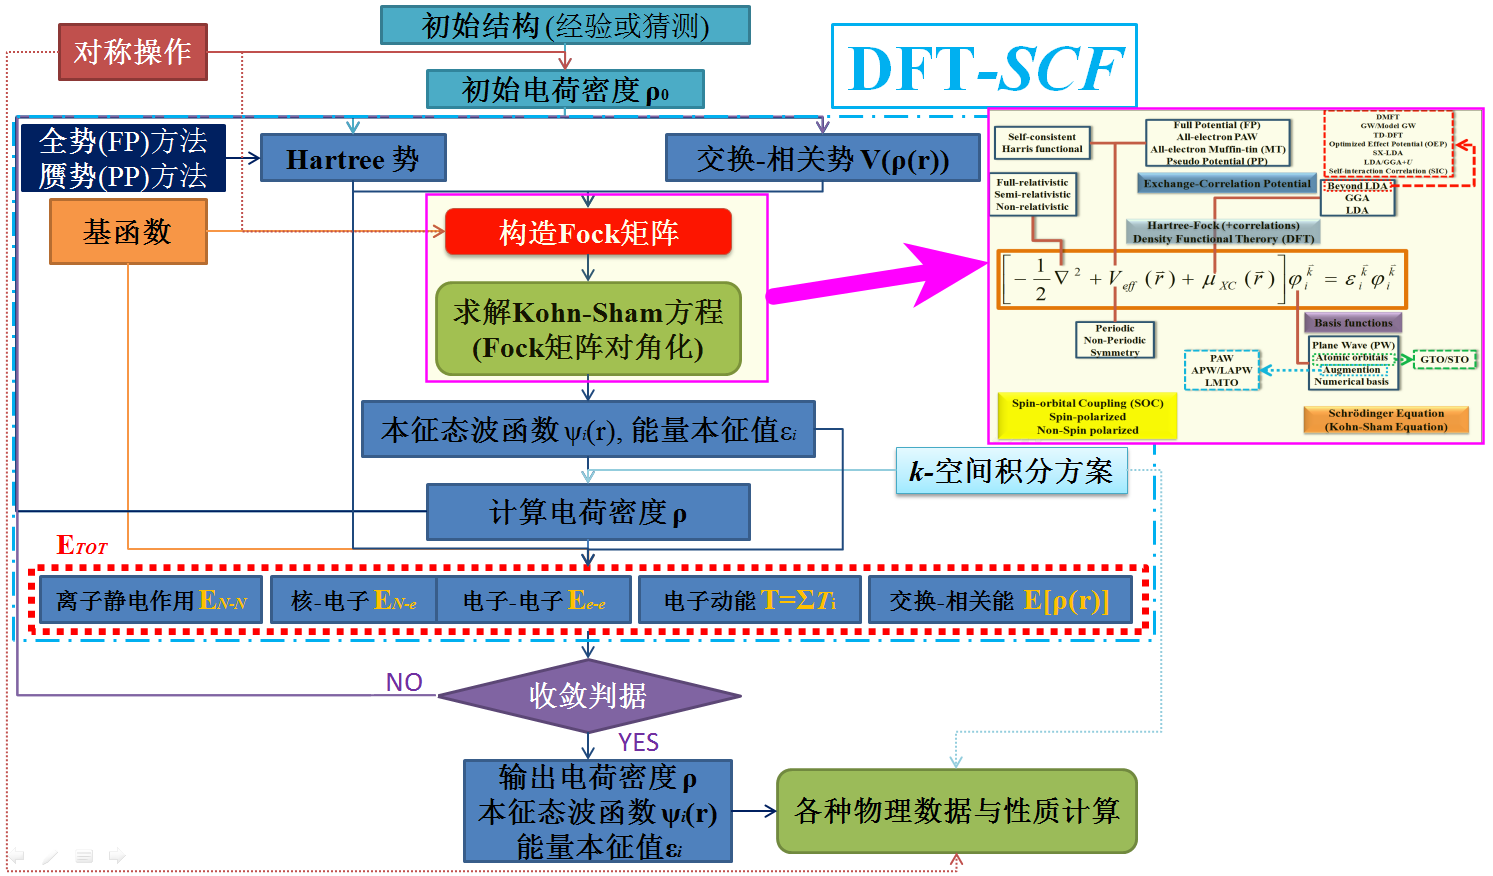
\includegraphics[height=2.80in,width=4.95in,viewport=5 3 1490 870,clip]{Figures/DFT-SCF_2.png}
%\caption{\small \textrm{Pseudopotential for metallic sodium, based on the empty core model and screened by the Thomas-Fermi dielectric function.}}%(与文献\cite{EPJB33-47_2003}图1对比)
\label{Pseudo-NC}
\end{figure}
}

%\section{Induction on DFT and solid-state physics}       %Bookmark
\section{平面波与赝势}       %Bookmark
\frame
{
	\frametitle{球形势对平面波的散射与相移}
\begin{figure}[h!]
\centering
\vspace*{-0.26in}
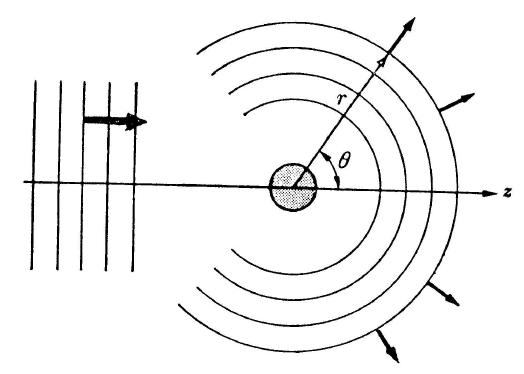
\includegraphics[height=0.90in,width=1.24in,viewport=0 0 400 300,clip]{Figures/Pseudo-scatter.jpg}
\caption{\small \textrm{Schematic illustration of scattering of a plane wave by a spherical potential.}}%(与文献\cite{EPJB33-47_2003}图1对比)
\label{Pseudo-scatter}
\end{figure}
$$\mathrm{e}^{\mathrm{i}\vec q\cdot\vec r}=4\pi\sum_{lm}\mathrm{i}^lj_l(\vec q\cdot\vec r)Y_{lm}^{\ast}(\hat{\vec q})Y_{lm}(\hat{\vec r})=\sum_{l}(2l+1)\mathrm{i}^lj_l(qr)P_{l}(\cos\theta)$$
%$$\mathrm{e}^{\mathrm{i}\vec q\cdot\vec r}=\mathrm{e}^{\mathrm{i}qr\cos(\theta)}=\sum_{l}(2l+1)\mathrm{i}^lj_l(qr)P_{l}[\cos(\theta)]$$
$$\Psi_l^{>}(\varepsilon,r)=C_l\bigg[j_l(\kappa r)-\tan\eta_l(\varepsilon)n_l(\kappa r)\bigg]\quad\text{其中}\kappa^2=\varepsilon$$
$$D_l(\varepsilon,r)\equiv r\psi_l^{\prime}(r)/\psi_l(r)=r\dfrac{\mathrm{d}}{\mathrm{d}r}\ln\psi_l(r)$$
$$\tan\eta_l(\varepsilon)=\dfrac{R\frac{\mathrm{d}}{\mathrm{d}r}j_l(\kappa r)|_R-D_l(\varepsilon)j_l(\kappa R)}{R\frac{\mathrm{d}}{\mathrm{d}r}n_l(\kappa r)|_R-D_l(\varepsilon)n_l(\kappa R)}$$
%$$t(\theta)=\dfrac{4\pi}{\sqrt\varepsilon}\sum_l(2l+1)\bigg[\mathrm{e}^{2\mathrm{i}\eta_l}-1\bigg]P_l(\cos\theta)$$
%$$\eta_l(\varepsilon)=p_l\pi+\delta_l(\varepsilon)$$
}

\frame
{
	\frametitle{散射相移与赝势}
\begin{figure}[h!]
\centering
\vspace*{-0.25in}
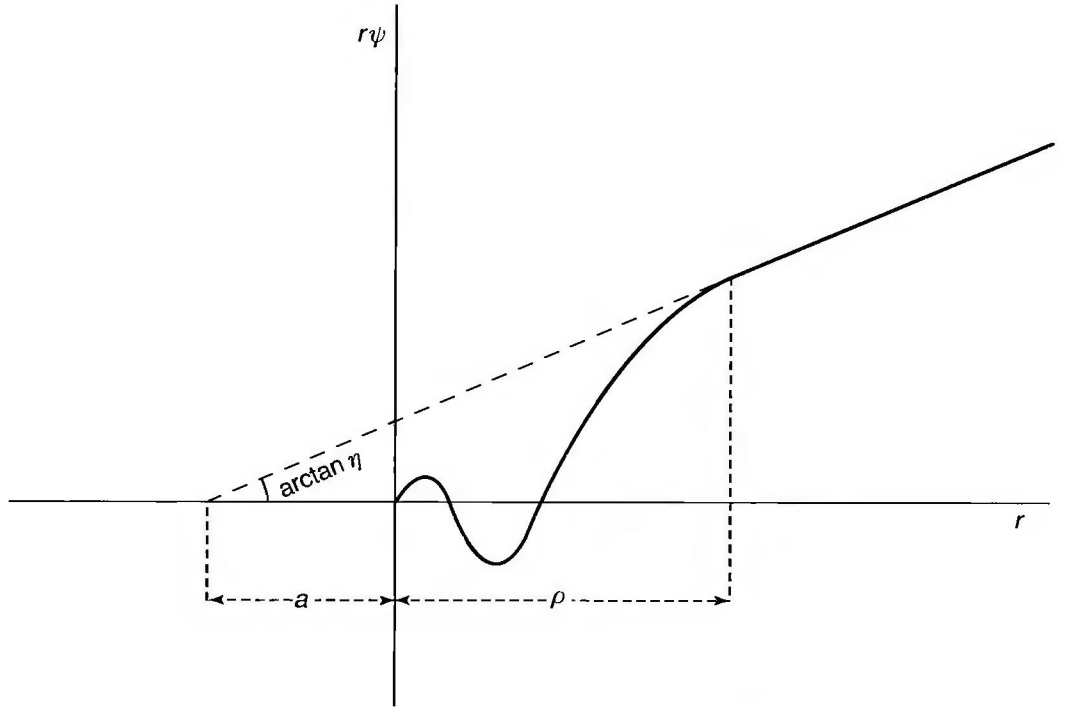
\includegraphics[height=1.50in,width=2.27in,viewport=0 0 1150 750,clip]{Figures/Pseudo-scatter-2.png}
\caption{{\footnotesize \textrm{Radial wave-function $\phi=r\psi$ for low-energy scattering as illustrated in a figure from the 1934 and 1935 papers of Fermi and coworkers for low-energy electron scattering from atoms and neutron scattering from nuclei. The node in the wave-function near the origin show that the potential is attractive and strong enough to have bound states. The cross-section for scattering from the localized potential is determined by the phase shift and is the same for weaker pseudo-potential with the same phase shift modulo $2\pi$.}}}%(与文献\cite{EPJB33-47_2003}图1对比)
\label{Pseudo-scatter-2}
\end{figure}
}

\frame
{
%\frametitle{The methods on band structure calculation}
\frametitle{由OPW到赝势}
%\vskip 10pt
%\textrm{The mainly difference of all these methods below: the basis sets and the construction of the potential}
\begin{itemize}
\setlength{\itemsep}{5pt}
	\item 完全平面波基组:~少数平面波就可以很好地描述波函数在原子间的行为,近核波函数则需要大量平面波展开。%因此完全平面波基组虽然方便,但求体系本征态对角化的矩阵非常巨大,计算变得异常耗时。
	\item 正交平面波(\textrm{Orthogonalized plane wave, OPW})方法,价电子用与芯层波函数正交的平面波展开
		\begin{displaymath}
			\phi_{OPW}^{\vec k+\vec G}(\vec r)=\phi_{PW}^{\vec k+\vec G}(\vec r)-\sum_c\langle\varphi_c|\phi_{PW}^{\vec k+\vec G}\rangle\varphi_c(\vec r)
		\end{displaymath}
		代入\textrm{Schr\"odinger}方程
		$$\hat H|\phi_{PW}^{\vec k+\vec G}\rangle-\sum_c\langle\varphi_c|\phi_{PW}^{\vec k+\vec G}\rangle\hat H|\varphi_c\rangle=\varepsilon|\phi_{PW}^{\vec k+\vec G}\rangle-\varepsilon\sum_c\langle\varphi_c|\phi_{PW}^{\vec k+\vec G}\rangle|\varphi_c\rangle$$
		可有$$\hat H|\phi_{PW}^{\vec k+\vec G}\rangle+\textcolor{blue}{V^R}|\phi_{PW}^{\vec k+\vec G}\rangle=\textcolor{blue}{\varepsilon}|\phi_{PW}^{\vec k+\vec G}\rangle$$
%		这里排斥势是$$V^R(\vec r,\vec r^{\prime})=\sum_c(\varepsilon-\varepsilon_c)|\varphi_c(\vec r^{\prime})\rangle\langle\varphi_c(\vec r)|$$
\end{itemize}
}

\frame
{
	\frametitle{由OPW到赝势}
	\textrm{Phillips-Kleinman}指出赝势($V^{eff}$)-赝波函数($\phi_{GW}^{\vec k+\vec G}$)满足\textrm{Schr\"odinger}方程\upcite{PR116_1959}
	$$\bigg(-\dfrac12\nabla^2+\textcolor{red}{V^{eff}}\bigg)|\phi_{GW}^{\vec k+\vec G}\rangle=\textcolor{blue}{\varepsilon}|\phi_{GW}^{\vec k+\vec G}\rangle$$
	其中$\textcolor{red}{V^{eff}}=V(\vec r)+\textcolor{blue}{V^R}$
	\begin{itemize}
		\item 赝势-赝波函数的本征值$\varepsilon$与真实体系的能量本征值等价
		\item 赝势$V^{eff}$比$V(\vec r)$平滑得多,并且$V^R$是非局域的排斥势
			\begin{displaymath}
				\begin{aligned}
					V^Rf(\vec r)=&\sum_c(\varepsilon-\varepsilon_c)\varphi_c(\vec r)\int\varphi_c^{\ast}(\vec r^{\prime})f(\vec r^{\prime})\mathrm{d}\vec r^{\prime} \\
					=&\int V^R(\vec r,\vec r^{\prime})f(\vec r^{\prime})\mathrm{d}\vec r^{\prime}
				\end{aligned}
			\end{displaymath}
			这里$$V^R(\vec r,\vec r^{\prime})=\sum_c(\varepsilon-\varepsilon_c)|\varphi_c(\vec r^{\prime})\rangle\langle\varphi_c(\vec r)|$$
	\end{itemize}
}

\frame
{
\frametitle{赝势方法}
赝势(\textrm{Pseudo Potential, PP})方法是在正交平面波的基础上发展起来的,构造出平缓的势函数代替核的强吸引作用和芯层电子的排斥作用,用平缓的函数取代波函数近核时的震荡。
\begin{itemize}
\setlength{\itemsep}{5pt}
	\item 赝势-平面波方法,只需要少量平面波可展开赝波函数,大大提升了计算效率;但是赝波函数不能很好地反映与电子近核行为有关的性质。
	\item 赝势的构造并不唯一,考核构造赝势的两大指标:~\\“柔软程度”\textrm{(Soft)}与“可移植性”\textrm{(transferability)}
\end{itemize}
\begin{figure}[h!]
\centering
\vspace*{-0.10in}
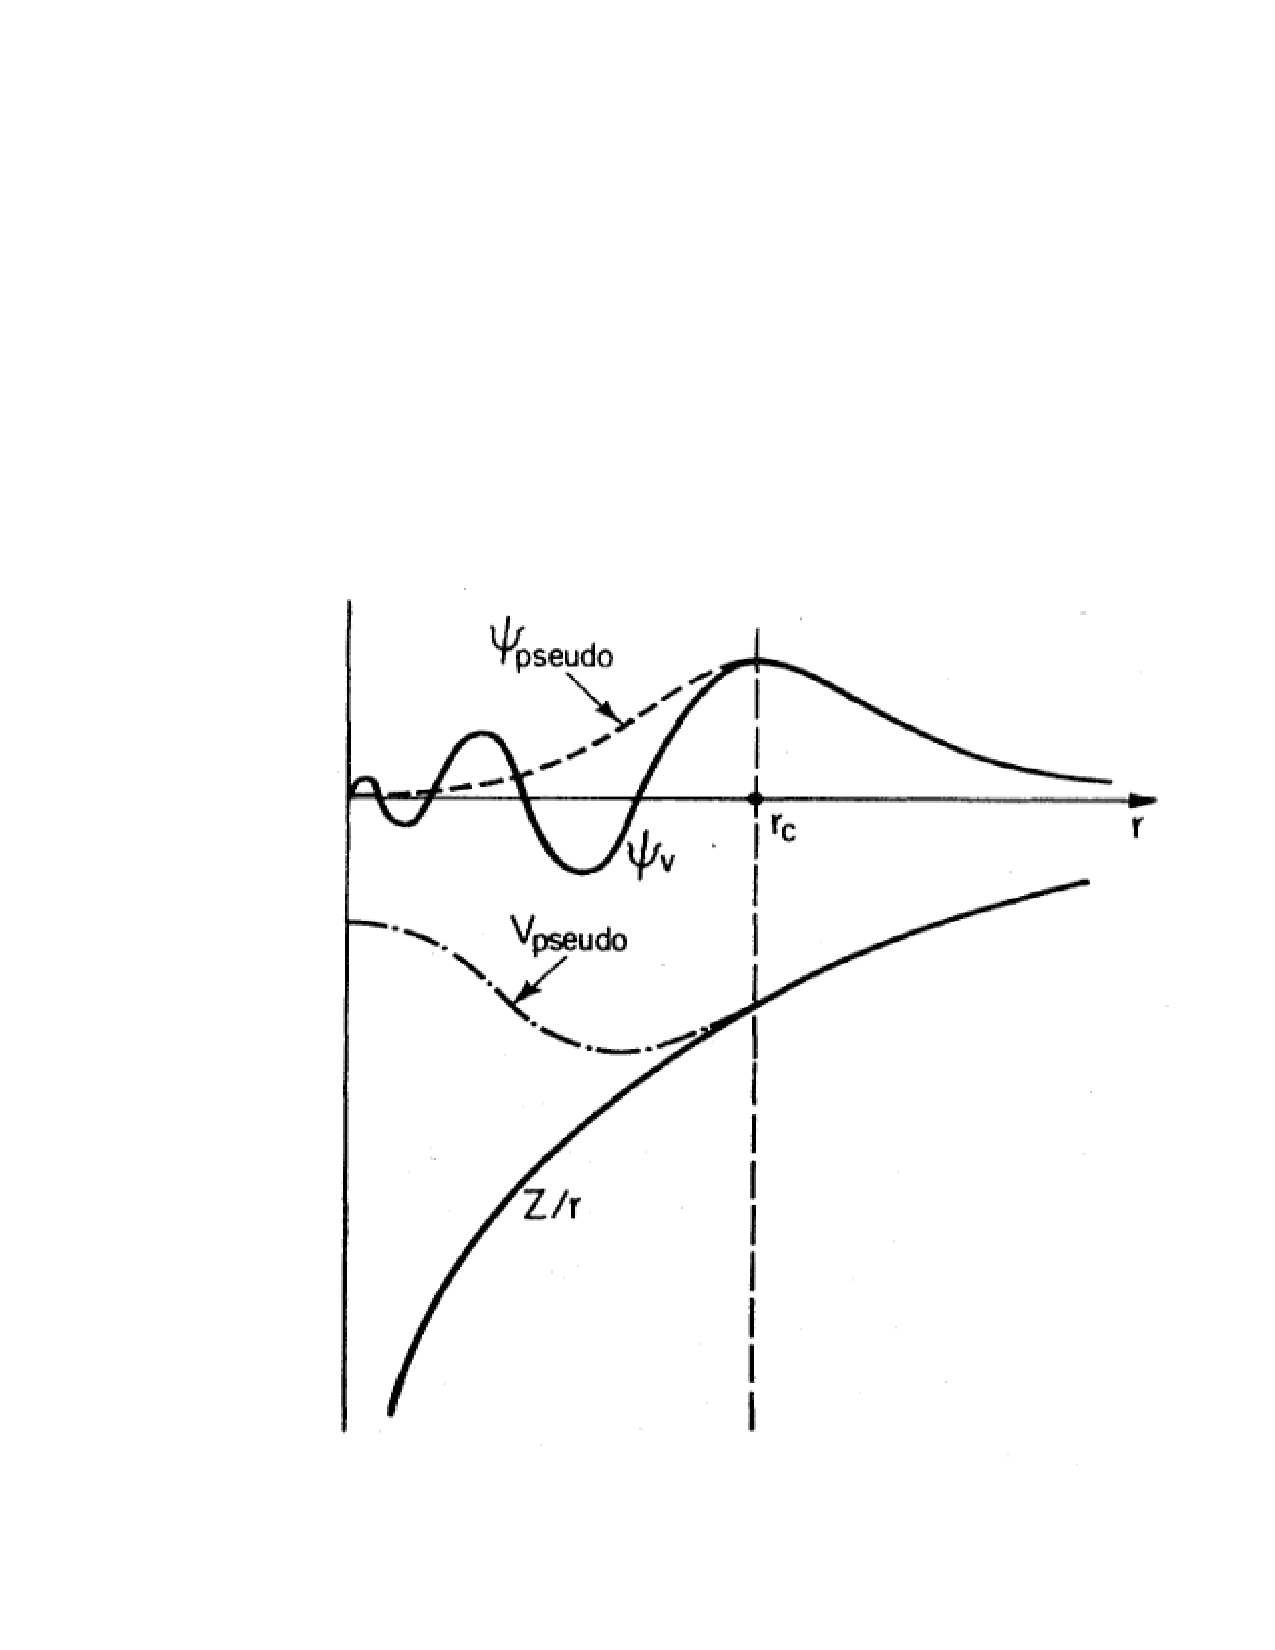
\includegraphics[height=1.35in,width=1.42in,viewport=154 100 562 508,clip]{Figures/Pseudo.pdf}
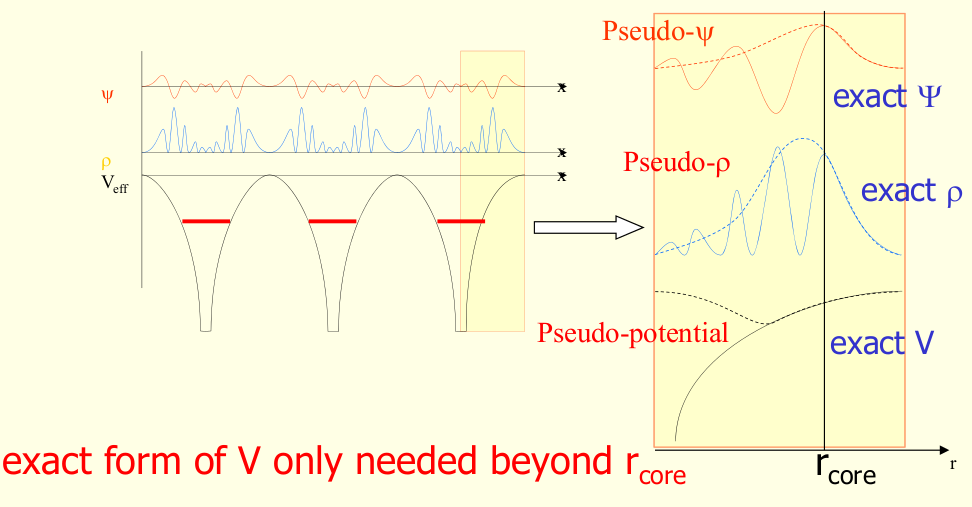
\includegraphics[height=1.35in,width=2.57in,viewport=1 1 980 500,clip]{Figures/Pseudo-2.png}
\caption{\small \textrm{The Pseudo wave function and Pseudo potential.}}%(与文献\cite{EPJB33-47_2003}图1对比)
\label{Pseudo_Potential-Wave}
\end{figure}
}

\section{模守恒赝势与超软赝势}
\frame
{
	\frametitle{传统赝势的构造}
	直接由实验数据来确定(模型)赝势,常用的实验数据包括离子对电子的散射角度、离子的光谱实验数据等
		\begin{itemize}
			\item 构造离子赝势:~可移植性好
			\item 构造总赝势(包括全部价电子相互作用):~常用于能带描述
		\end{itemize}
%	\begin{itemize}
%		\item 在指定能量范围内,离子对电子散射的散射角
%		\item 离子的光谱实验数据
%	\end{itemize}
\begin{figure}[h!]
\centering
\vspace*{-0.10in}
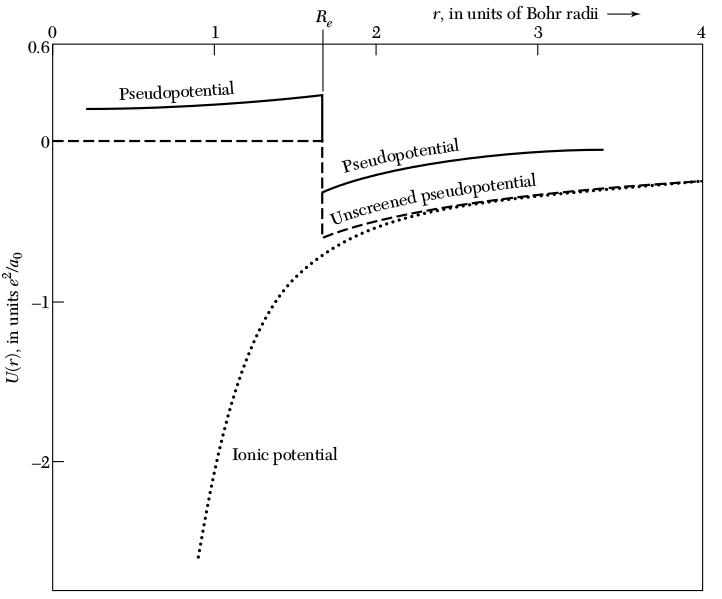
\includegraphics[height=1.60in,width=2.57in,viewport=0 0 980 600,clip]{Figures/Pseudo-model-empty_core.png}
\caption{\small \textrm{Pseudopotential for metallic sodium, based on the empty core model and screened by the Thomas-Fermi dielectric function.}}%(与文献\cite{EPJB33-47_2003}图1对比)
\label{Pseudo_model-empty_core}
\end{figure}
}

\frame
{
	\frametitle{传统赝势的构造}
\begin{figure}[h!]
\centering
\vspace*{-0.10in}
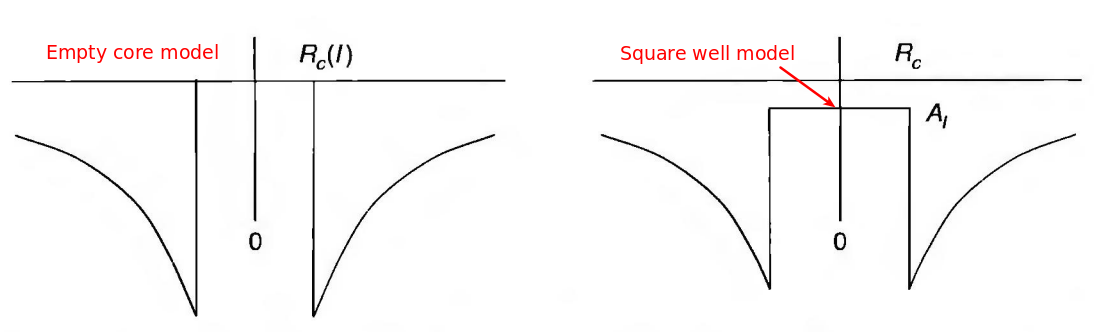
\includegraphics[height=1.30in,width=4.17in,viewport=0 0 1150 350,clip]{Figures/Pseudo-model.png}
\caption{\small \textrm{Left:``Empty core'' model potential of Ashcroft in which the potential is zero inside radius $R_c(l)$ which is different for each $l$. Right: Square well model potential with value $A_l$ inside a cut-off radius $R_c$, proposed by Abarenkov and Heine and fit to atomic data by Animalu and Heine. THe fact that the potential are weak, zero, or even positive inside cut-off radius $R_c$ is an illustration of the ``cancellation theorem''.}}%(与文献\cite{EPJB33-47_2003}图1对比)
\label{Pseudo-model}
\end{figure}
}

\frame
{
	\frametitle{第一原理赝势}
		由第一原理求解出全电子波函数(径向部分)$P_{n,l}(r)$
			\begin{displaymath}
				\bigg[-\dfrac12\dfrac{\mathrm{d}^2}{\mathrm{d}r^2}+\dfrac{l(l+1)}{2r^2}+V(\rho,r)\bigg]P_{n,l}(r)=\varepsilon_{n,l}P_{n,l}(r)
			\end{displaymath}
			这里$V(\rho,r)$是自洽单电子势
			$$V(\rho,r)=-\frac{Z}r+V_{\mathrm H}(\rho,r)+V_{XC}^{\mathrm{LDA}}(\rho(r))$$
			$V_{\mathrm H}(\rho,r)$是\textrm{Hartree}势,$V_{XC}^{\mathrm{LDA}}(\rho(r))$是交换-相关势

			由此构造赝波函数$P_l^{\mathrm{PP}}(r)$,满足
			$$P_l^{\mathrm{PP}}(r)=P_l^{\mathrm{AE}}(r),\quad r>r_{cl}$$
			进而构造赝势$V_{\mathrm{src},l}^{\mathrm{PP}}(r)$
			$$V_{\mathrm{src},l}^{\mathrm{PP}}(r)=\varepsilon_l-\dfrac{l(l+2)}{2r^2}+\dfrac{1}{2P_l^{\mathrm{PP}}(r)}\dfrac{\mathrm{d}^2}{\mathrm{d}r^2}P_l^{\mathrm{AE}}(r),\quad r>r_{cl}$$
}

\frame
{
	\frametitle{模守恒\textrm{(Norm-conserving)}条件}
%	构造赝势确定参数的边界(构造条件)
	\begin{enumerate}
		\item 价电子赝波函数的能量本征值与对应全电子波函数能量本征值相等:~$\varepsilon_l^{\mathrm{PP}}=\varepsilon_l^{\mathrm{AE}}$
		\item 价电子赝波函数与真实电子波函数的径向部分在截断半径$r_{c,l}$外相同:~$\psi_l^{\mathrm{PP}}(r)=\psi_l^{\mathrm{AE}}(r),\quad r>r_{cl}$
		\item 价电子赝波函数与真实电子波函数的对数导数在截断半径$r_{c,l}$处相等:~$D_l^{\mathrm{PP}}(r)=D_l^{\mathrm{AE}}(r),\quad r\geqslant r_{cl}$\\
		这里$D_l(\varepsilon,r)=r\frac{\psi_l^{\prime}(\varepsilon,r)}{\psi_l(\varepsilon,r)}=r\dfrac{\mathrm{d}}{\mathrm{d}r}\ln\psi_l(\varepsilon,r)$
		\item 价电子赝波函数与真实电子波函数在截断半径$r_{c,l}$内的积分电荷相等(\textcolor{red}{模守恒条件})
			$$Q_l=\int_0^{r_{cl}}\mathrm{d}rr^2|\psi_l^{\mathrm{PP}}(r)|^2=\int_0^{r_{cl}}\mathrm{d}rr^2|\psi_l^{\mathrm{AE}}(r)|^2$$
		\item 价电子赝波函数与真实电子波函数的对数导数一阶能量导数$\mathrm{d}D_l(\varepsilon,r)/\mathrm{d}\varepsilon$在截断半径$r_{c,l}$处及以外相等
	\end{enumerate}
}

\frame
{
	\frametitle{模守恒\textrm{(Norm-conserving)}条件}
\begin{figure}[h!]
\centering
\vspace*{-0.10in}
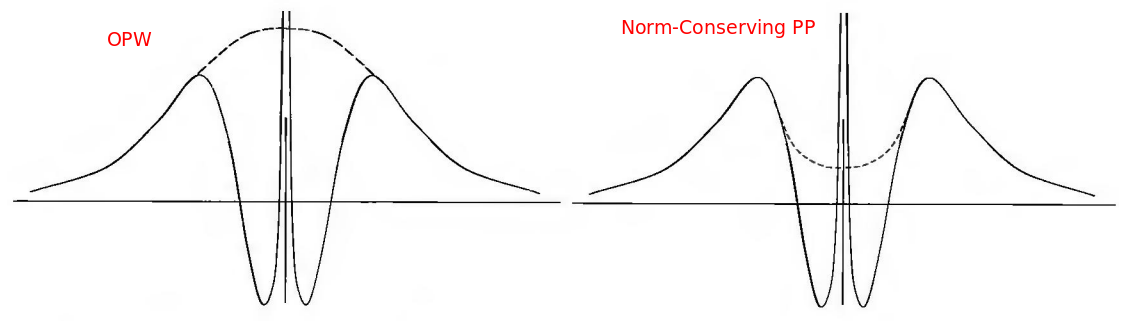
\includegraphics[height=1.30in,width=4.17in,viewport=0 0 1150 350,clip]{Figures/Pseudo-OPW_NCPP.png}
\caption{\small \textrm{Schematic example of a valence function that has the character of a $3s$ orbital near the nucleus and two examples of smooth functions (dashed lines) that equal the full wave-function outside the core region. Left: the smooth part of the valence function defined by OPW-like equation; Right: a smooth pseudo-function that satisfies the norm-conservation condition.}}%(与文献\cite{EPJB33-47_2003}图1对比)
\label{Pseudo-OPW_NCPP}
\end{figure}
}

\frame
{
	\frametitle{赝势去屏蔽与非局域化}
	第一原理赝势建立了赝波函数与对应赝势的一一对应关系,但该赝势包含了电子屏蔽(原子、离子环境)信息,去屏蔽后的赝势对环境依赖更低,“可移植性”更好
	$$V_{\mathrm{ion},l}^{\mathrm{PP}}(r)=V_{\mathrm{src},l}^{\mathrm{PP}}(r)-V_{\mathrm{H},l}^{\mathrm{PP}}(r)-V_{XC,l}^{\mathrm{PP}}(r)$$
	去屏蔽过程中,特别需要注意$V_{XC,l}^{\mathrm{PP}}(r)$的处理
	$$V_{XC}^{\mathrm{PP}}(r)=V_{XC}^{\mathrm{PP}}([n^{\mathrm{PP}}],r)+\big[V_{XC,l}^{\mathrm{PP}}([n^{\mathrm{PP}}+n^{core}],r)-V_{XC}^{\mathrm{PP}}([n^{\mathrm{PP}}],r)\big]$$
	如果定义函数
	$$\chi_{lm}^{\mathrm{PP}}(\vec r)=\bigg\{\varepsilon_l-\bigg[-\dfrac12\nabla^2+V_{local}^{\mathrm{PP}}(\vec r)\bigg]\bigg\}\psi_{lm}^{\mathrm{PP}}(\vec r)$$
	赝势可以分解为局域部分与非局域部分之和
	$$V_{NL}^{\mathrm{PP}}(r)=V_{local}^{\mathrm{PP}}(r)+\dfrac{|\chi_{lm}^{\mathrm{PP}}\rangle\langle\chi_{lm}^{\mathrm{PP}}|}{\langle\chi_{lm}^{\mathrm{PP}}|\psi_{lm}^{\mathrm{PP}}\rangle}=V_{local}^{\mathrm{PP}}(r)+\sum_{lm}\dfrac{|\psi_{lm}^{\mathrm{PP}}\delta V_l\rangle\langle\delta V_l\psi_{lm}^{\mathrm{PP}}|}{\langle\psi_{lm}^{\mathrm{PP}}|\delta V_l|\psi_{lm}^{\mathrm{PP}}\rangle}$$
}

\frame
{
	\frametitle{模守恒赝势构造流程}
\begin{figure}[h!]
\centering
%\vspace*{-0.10in}
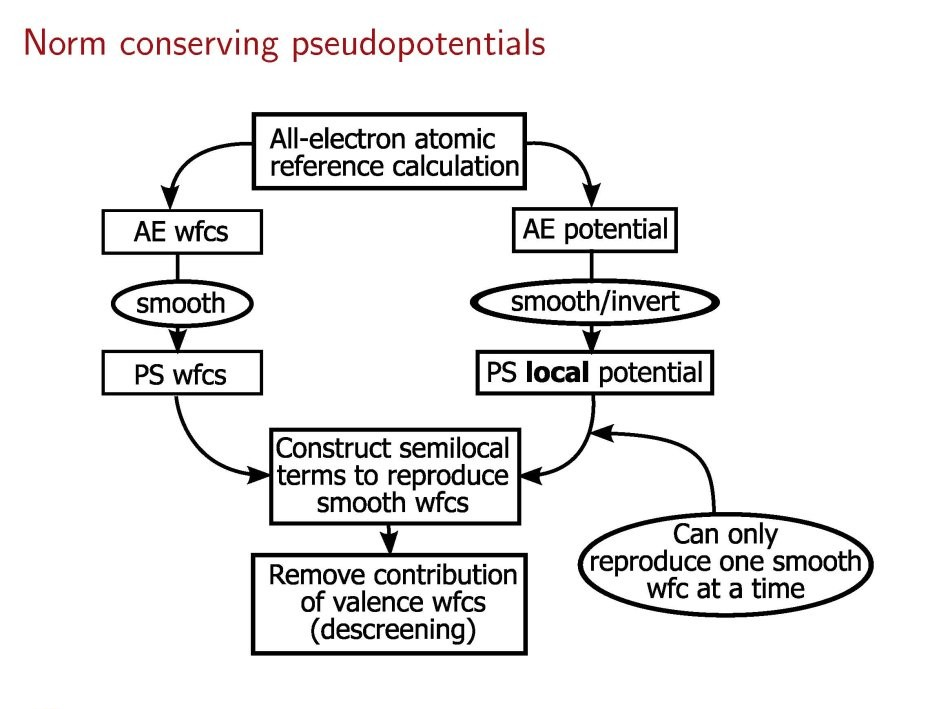
\includegraphics[height=2.70in,width=3.77in,viewport=70 40 900 610,clip]{Figures/Pseudo-NC.jpg}
%\caption{\small \textrm{Pseudopotential for metallic sodium, based on the empty core model and screened by the Thomas-Fermi dielectric function.}}%(与文献\cite{EPJB33-47_2003}图1对比)
\label{Pseudo-NC}
\end{figure}
}

\frame
{
\frametitle{超软赝势}
\begin{itemize}
\setlength{\itemsep}{5pt}
	\item 赝势构造的模守恒条件
%		\begin{displaymath}
%			\int_0^{r_c}\mathrm{d}\vec r\varphi^{\ast PS}(\vec r)\varphi^{PS}(\vec r)=\int_0^{r_c}\mathrm{d}\vec r\varphi^{\ast}(\vec r)\varphi(\vec r)
%		\end{displaymath}
	很好地解决了赝势可移植性问题,但对$1s$、$2p$、$3d$等轨道,模守恒方案构造的赝势过于“硬”,所需平面波基组依然非常大
	\item 超软\textrm{(Ultra-soft)}赝势,解除模守恒条件,实现对第一、第二周期元素的高效计算
\end{itemize}
\begin{figure}[h!]
\vspace*{-0.10in}
\centering
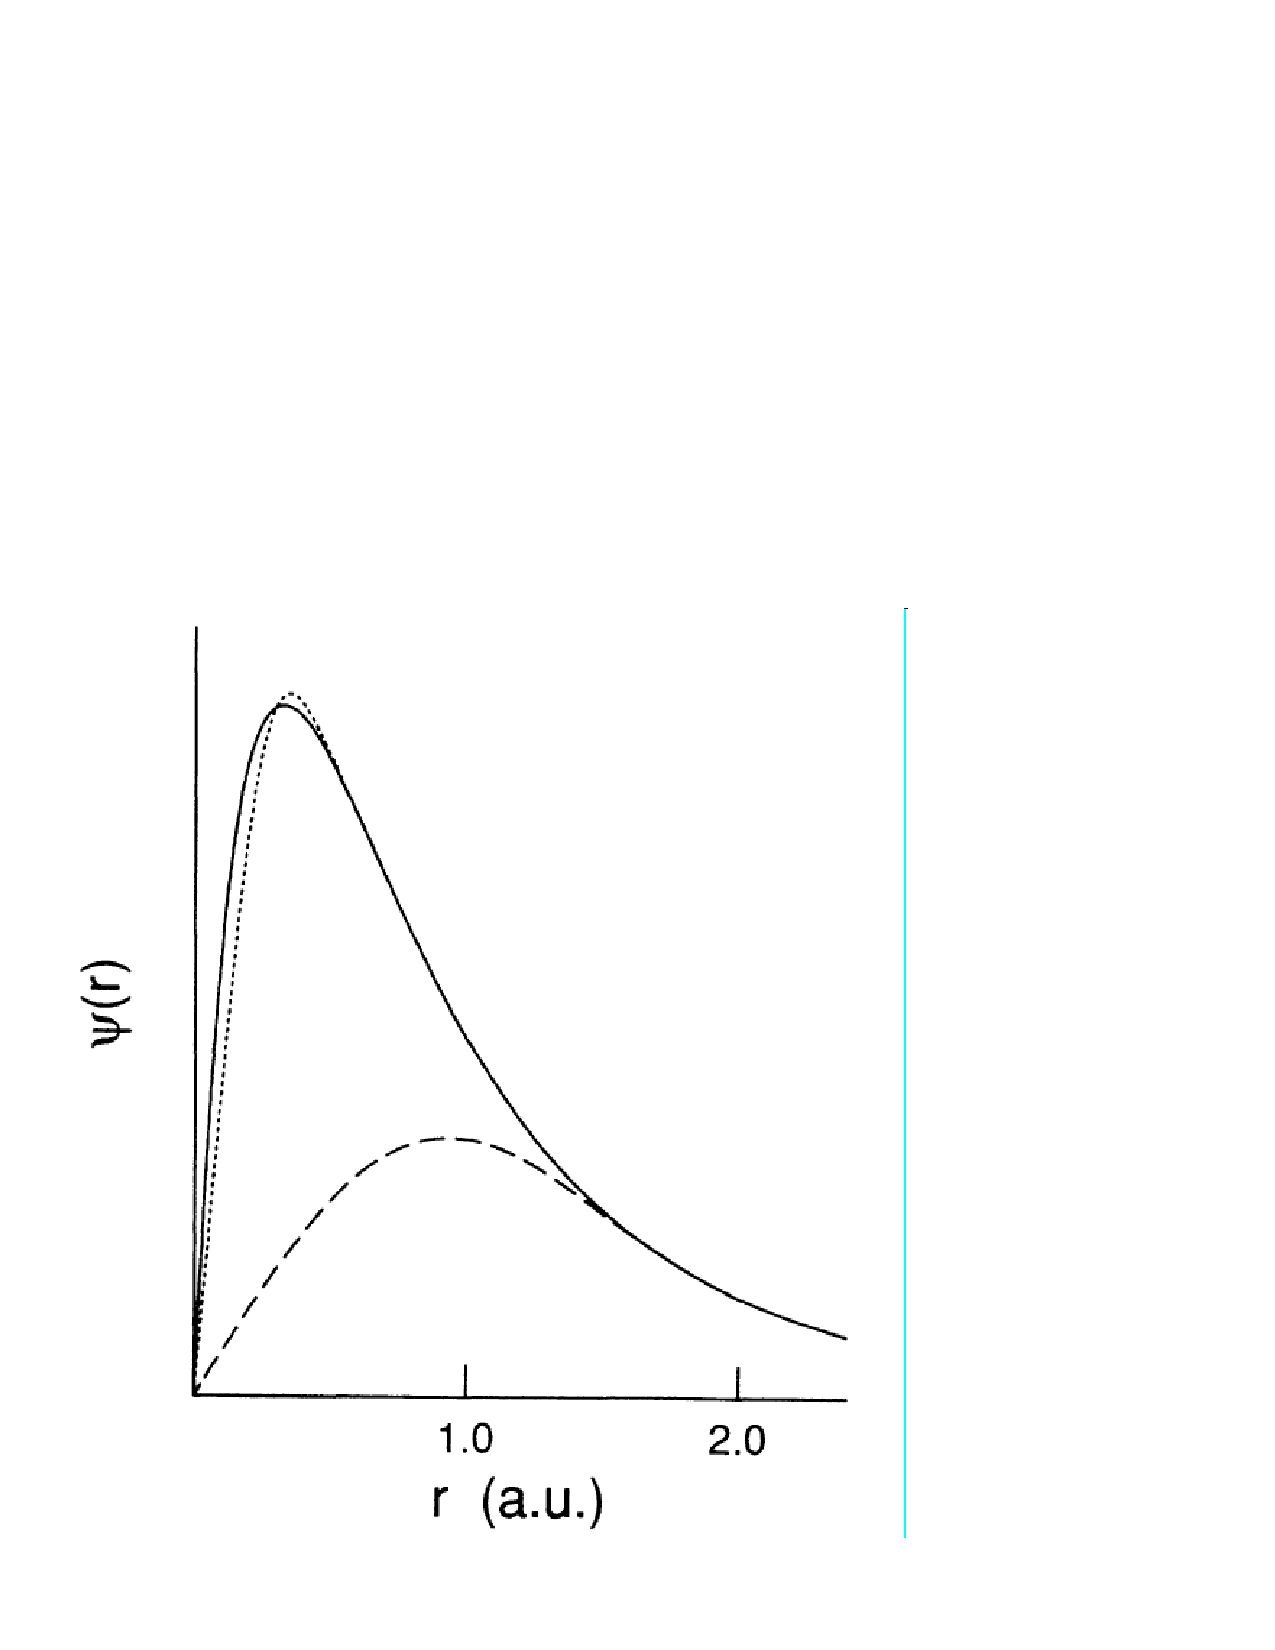
\includegraphics[height=1.35in,width=1.40in,viewport=30 55 415 500,clip]{Figures/Norm-US-wave.pdf}
\caption{\small \textrm{Oxygen 2} \textit{p} \textrm{radical wave function (solid), NC-pseudo-wave (dottde) and US-pseudo-wave (dashed).}}%(与文献\cite{EPJB33-47_2003}图1对比)
\label{Norm-US-wave}
\end{figure}
}

\frame
{
\frametitle{超软赝势的构造}
超软赝势在平缓的局域势函数$V^L(\vec r)$和赝波函数$|\phi_{lmj}(\vec r)\rangle$的基础上,构造函数
\begin{displaymath}
	|\chi_{lmj}(\vec r)\rangle=\bigg[\varepsilon_{lj}-\dfrac12\nabla^2-V^L(\vec r)\bigg]|\phi_{lmj}(\vec r)\rangle
\end{displaymath}
在此基础上得到矩阵$\mathbf{D}_{ij}=\langle\phi_i|\chi_j\rangle$和局域函数
\begin{displaymath}
	|\beta_i\rangle=\sum_j(\mathbf{D}^{-1})_{ji}|\chi_{j}\rangle
\end{displaymath}
因此非局域赝势可以表示为
\begin{displaymath}
	V_{NL}=\dfrac{|\chi_i\rangle\langle\chi_i|}{\langle\chi_i|\phi_i\rangle}=\sum_{i,j}\mathbf{D}_{ij}|\beta_i\rangle\langle\beta_j|
\end{displaymath}
用平缓函数构造赝波函数与真实波函数的电荷密度差
\begin{displaymath}
	Q_{nm}(\vec r)=\varphi_n^{\ast}(\vec r)\varphi_m(\vec r)-\tilde\varphi_n^{\ast}(\vec r)\tilde\varphi_m(\vec r)
\end{displaymath}
}

\frame
{
	\frametitle{超软赝势总能量计算}
	\begin{displaymath}
		\begin{aligned}
			E_{\mathrm{total}}=&\sum_j^{\mathrm{occ}}\langle\phi_{lmj}|\bigg[-\dfrac12\nabla^2+V_{\mathrm{local}}^{\mathrm{ion}}+\sum_{s,s^{\prime}}\mathbf{D}_{s,s^{\prime}}^{\mathrm{ion}}|\beta_s\rangle\langle\beta_{s^{\prime}}|\bigg]|\phi_{lmj}\rangle\\
			&+E_{H}[n_v]+E_{N-N}+E_{XC}[n_v]
		\end{aligned}
	\end{displaymath}
	其中$n_v(\vec r)=\sum\limits_j^{\mathrm{occ}}\phi_{lmj}^{\ast}(\vec r)\phi_{lmj}(\vec r)+\sum\limits_{s,s^{\prime}}\sum\limits_j^{\mathrm{occ}}\langle\phi_{lmj}|\beta_{s^{\prime}}\rangle\langle\beta_s|\phi_{lmj}\rangle Q_{s,s^{\prime}}(\vec r)$
	$$V_{\mathrm{local}}^{\mathrm{ion}}=V_{local}-V_{\mathrm H}-V_{XC}$$
	$$\mathbf{D}_{s,s^{\prime}}^{\mathrm{ion}}=\mathbf{D}_{s,s^{\prime}}-\int\mathrm{d}\vec r\big[V_{\mathrm{H}}(\vec r)+V_{XC}(\vec r)\big]Q_{s,s^{\prime}}(r)$$
	由此可得广义本征值方程
	$$\bigg[-\dfrac12\nabla^2+V_{\mathrm{local}}+V_{NL}^{\mathrm{US}}-\varepsilon_i\bigg(\mathbf{1}+\sum_{s,s^{\prime}}Q_{s,s^{\prime}}|\beta_s\rangle\langle\beta_{s^{\prime}}|\bigg)\bigg]|\phi_{lmi}\rangle=0$$
}

\appendix
\frame
{
	\frametitle{赝势生成程序\textrm{Atompaw}的计算细节}
	求解原子的价层的全电子分波函数
	$$\hspace*{-62pt}{\footnotesize\bigg(-\dfrac{\hbar^2}{2m}\nabla^2-\dfrac{Ze^2}r+e^2\int\mathrm{d}^3r^{\prime}\dfrac{n_{core}(r^{\prime})+n(r^{\prime})}{|r-r^{\prime}|}+\mu_{XC}[n_{core}(r)+n(r)]\bigg)|\phi_i\rangle=\epsilon_i|\phi_i\rangle}$$
	全电子分波电荷密度
	$$n(r)=\sum_{n,l}c_{n,l}\dfrac{|\phi_{n,l}(r)|^2}{4\pi r^2}$$
}

\frame
{
	\frametitle{赝势生成程序\textrm{Atompaw}的计算细节}
	有效赝势的构造方案
	\begin{itemize}
		\item \textrm{Troullier-Martin NC} 方案 \\
	首先构造赝波函数满足
	\begin{displaymath}
		\tilde\phi(r)=\left\{
			\begin{aligned}
				&r^{L_v+1}\mathrm{e}^{p(r)}\quad &\mathrm{for}\quad r\leqslant r_c \\
				&\phi(r)\quad &\mathrm{for}\quad r>r_c
			\end{aligned}
			\right.
	\end{displaymath}
	这里$$p(r)=\sum_{m=0}^6C_mr^{2m}$$
	可得赝势 
	$$V_{eff}^{PS}(r)=\epsilon_l+\dfrac{\hbar^2}{2m}\bigg(\dfrac{\mathrm{d}^2p}{\mathrm{d}r^2}+(\dfrac{\mathrm{d}p}{\mathrm{d}r})^2+\dfrac{2(L_v+1)}r\dfrac{\mathrm{d}p}{\mathrm{d}r}\bigg)$$
	于是赝\textrm{Hamiltonian}是$\tilde H(r)=-\dfrac{\hbar^2}{2m}\nabla^2+V_{eff}^{PS}(r)$
	\end{itemize}
}
\frame
{
	\frametitle{赝势生成程序\textrm{Atompaw}的计算细节}
	有效赝势的构造方案
	\begin{itemize}
		\item \textrm{Ultra-soft} 方案 \\
	构造赝波函数满足
	\begin{displaymath}
		\tilde\phi(r)=\left\{
			\begin{aligned}
				&r^{L_v+1}\sum_{m=0}^3C_mr^{2m}\quad &\mathrm{for}\quad r\leqslant r_c \\
				&\phi(r)\quad &\mathrm{for}\quad r>r_c
			\end{aligned}
			\right.
	\end{displaymath}
	与\textrm{Troullier-Martin NC}方案类似,逆向求解本征方程得到有效赝势
		\item \textrm{Bessel}方案\\
			直接构造有效赝势 $V_{eff}^{PS}(r)=\alpha\cdot\dfrac{\sin(q\cdot r)}r$
	\end{itemize}
}

\frame
{
	\frametitle{赝势生成程序\textrm{Atompaw}的计算细节}
	赝分波函数与投影子函数构造
	\begin{itemize}
		\item \textrm{Bl\"ochl}方法\\
			构造截断函数$k(r)$
	\begin{displaymath}
		k(r)=\left\{
			\begin{aligned}
				&\bigg[\dfrac{\sin({\pi r/r_c})}{(\pi r/r_c)}\bigg]^2\qquad &\mathrm{for}\quad r<r_c \\
				&0\qquad &\mathrm{for}\quad r\geqslant r_c
			\end{aligned}
			\right.
	\end{displaymath}
	迭代求解方程
	$$(\tilde H(\vec r)-\epsilon_i)|\tilde\phi_i^0(\vec r)\rangle=C_ik(r)|\phi_i^0(\vec r)\rangle$$
	得到初始赝分波$\phi_i^0(\vec r)$\\
	初始投影子函数$|\tilde p_i^0(\vec r)\rangle=\dfrac{k(r)|\tilde\phi_i^0(\vec r)\rangle}{\langle\phi_i^0|k|\phi_i^0\rangle}$
	采用\textrm{Gram-Schmidt}正交化方法正交
	\end{itemize}
}

\frame
{
	\frametitle{赝势生成程序\textrm{Atompaw}的计算细节}
	赝分波函数与投影子函数构造
	\begin{itemize}
		\item \textrm{Vanderbilt}方法\\
			用多项式构造赝分波函数
	\begin{displaymath}
		\tilde\phi_i(r)=\left\{
			\begin{aligned}
				&r^{l+1}\sum_{m=0}^4C_mr^{2m}\qquad &\mathrm{for}\quad r<r_c \\
				&\phi_l(r)\qquad &\mathrm{for}\quad r\geqslant r_c
			\end{aligned}
			\right.
	\end{displaymath}
	构造辅助函数
	$$\chi_l(r)=\bigg(\epsilon_l+\dfrac{\hbar^2}{2m}(\dfrac{\mathrm{d}^2}{\mathrm{d}r^2}-\dfrac{l(l+1)}{r^2}-V_{eff}^{PS}(r)\bigg)\tilde\phi_l(r)$$
	和变换矩阵\textbf{B},矩阵元$B_{ij}=\int_0^{r_c}\mathrm{d}r\tilde\phi_i(r)\chi_j(r)$
	由此得到投影子函数$\tilde p_i(\vec r)=\sum_{j}\chi_j(r)(\mathbf{B^{-1}})_{ji}$
	\end{itemize}
}


\frame
{
	\frametitle{赝势生成程序\textrm{Atompaw}的计算细节}
	赝分波函数与投影子函数构造
	\begin{itemize}
		\item \textrm{RRKJ}方法\\
		构造赝分波函数
	\begin{displaymath}
		\tilde\phi_i=\left\{
			\begin{aligned}
				&r\cdot\bigg[\alpha_1^l\cdot j_l(q_1^lr)+\alpha_2^l\cdot j_l(q_2^lr)\bigg] \qquad &\mathrm{for}\quad r<r_c \\
				&\phi_l(r)\qquad &\mathrm{for}\quad r\geqslant r_c
			\end{aligned}
			\right.
	\end{displaymath}
	投影子函数的构造与\textrm{Vanderbilt}方法类似
	\end{itemize}
}


\frame
{
	\frametitle{赝势生成程序\textrm{Atompaw}的计算细节}
	\begin{itemize}
		\item 赝分波电荷密度的计算
	$$\tilde n(r)=\sum_{n,l}c_{n,l}\dfrac{|\tilde\phi_{n,l}(r)|^2}{4\pi r^2}$$
		\item 赝芯波电荷密度的计算
	\begin{displaymath}
		4\pi r^2\tilde n_{core}(r)=\left\{
			\begin{aligned}
				&r^2(U_0+U_2r^2+U_4r^4)\quad &\mathrm{for}\quad r\leqslant r_c \\
				&4\pi r^2n_{core}(r)\quad &\mathrm{for}\quad r>r_c
			\end{aligned}
			\right.
	\end{displaymath}
	\end{itemize}
}

%\frame
%{
%\frametitle{发展统一理论框架下的材料计算程序}
%\begin{itemize}
%	\item
%\end{itemize}
%}

\appendix
%------------------------------------------------------------------------Reference----------------------------------------------------------------------------------------------
%\begin{thebibliography}{99}
%-----------------------------------------------------------------------------------------------------------------------------------------------------------------------%
%\frame
%{
%\frametitle{主要参考文献}
%{\small
%\bibitem{Singh_Book}\textrm{D. J. Singh. \textit{Plane Wave, PseudoPotential and the LAPW method} (Kluwer Academic, Boston,USA, 1994)}					%
%  \nocite{*}																				%
%}
%}
%\end{thebibliography}
\begin{thebibliography}{99}
\frame
{
\frametitle{主要参考文献}
{\small
	\bibitem{PR57-1169_1940}\textrm{C. Herring. \textit{Phys. Rev.}, \textbf{57} (1940), 1169}
        \bibitem{Singh_Book}\textrm{D. J. Singh. \textit{Plane Wave, PseudoPotential and the LAPW method} (Kluwer Academic, Boston,USA, 1994)}
	\bibitem{PR116_1959}\textrm{J. C. Phillips and L. Kleinman. \textit{Phys. Rev.} (1959), 116}
	\bibitem{PRL43-1494_1979}\textrm{D. R. Hamann, M. Schl\"uter and C. Chiang. \textit{Phys. Rev. Lett.} \textbf{43} (1979), 1494}
        \bibitem{PRB41-7892_1990}\textrm{D. Vanderbilt. \textit{Phys. Rev.} B, \textbf{41} (1990), 7892} 
        \bibitem{JPCM6-8245_1994}\textrm{G. Kresse and J. Hafner. J. Phys: \textit{Condens. Matter}, \textbf{6} (1994), 8245}
%        \bibitem{PRB50-17953_1994}\textrm{P. E. Bl\"ochl. \textit{Phys. Rev.} B, \textbf{50} (1994), 17953}
%        \bibitem{PRB59-1758_1999}\textrm{G. Kresse and D. Joubert \textit{Phys. Rev.} B, \textbf{59} (1999), 1758}
	\bibitem{Elect_Stru}\textrm{Richard. M. Martin. \textit{Electronic Structure: Basic Theory and Practical Methods} (Cambridge University Press, Cambridge, England, 2004)}
}
\nocite*{}
}
\end{thebibliography}
%{\small
%\phantomsection\addcontentsline{toc}{section}{Bibliography}	 %直接调用\addcontentsline命令可能导致超链指向不准确,一般需要在之前调用一次\phantomsection命令加以修正	%
%\bibliography{Myref}																			%
%\bibliographystyle{mybib}																		%
%  \nocite{*}																				%
%}
%-----------------------------------------------------------------------------------------------------------------------------------------------------------------------%


%-----------------------------------------------------------Beamer下不建议使用bib,因为涉及分页--------------------------------------------------------------------------%
%{\small
%\phantomsection\addcontentsline{toc}{section}{Bibliography}	 %直接调用\addcontentsline命令可能导致超链指向不准确,一般需要在之前调用一次\phantomsection命令加以修正	%
%\bibliography{Myref}																			%
%\bibliographystyle{mybib}																		%
%  \nocite{*}																				%
%}

%------------------------------------------------------------------------------------------------------------------------------------------------------------------------------%

%-------------------------------------------------------------------------Thanks------------------------------------------------------------------------------------------------
%\section{致谢}
%\frame
%{
%\frametitle{致$\quad$谢}
%\begin{itemize}
%    \setlength{\itemsep}{20pt}
%  \item 感谢本团队高兴誉、吴泉生、宋红州等各位老师参与的讨论
%  \item 感谢莫所长、宋主任以及软件中心各位老师和同事
%  \item 感谢王崇愚先生的帮助
%\end{itemize}
%}
\frame
{
\vskip 60 pt
%\hskip 10pt \textcolor{blue}{\Huge 感谢答辩委员会各位老师\,\textrm{!}}\\
\vskip 35 pt
\hskip 60pt \textcolor{blue}{\Huge 谢谢大家\:!}
%\vskip 15 pt
%\hskip 40pt \textcolor{blue}{\Huge \textrm{for your attention\:!}}
}

%-------------------------------------------------------------------------------------------------------------------------------------------------------------------------------

\clearpage
%\end{CJK*}
\end{document}
